\chapter{Data}\label{sec-3.data}

We conduct our empirical research using various data sources: (1) detailed transaction data from China’s Custom Database, (2) the Chinese Industrial Enterprises from the National Bureau of Statistics of China, and (3) country-level macro data from Penn World Table 10.0. In this section, we will introduce the basic information of these datasets.

\section{Customs transaction records}

The main dataset we use is the transaction level records from the General Administration of Customs of China (GACC) as in Manova and Zhang (2012)\cite{manova-zhang2012}. The sample in this paper ranges from 2000 to 2011. This dataset includes the most comprehensive information on all Chinese trade transactions including import and export values (denominated in US dollars), quantities, quantity units, product names and codes, source and destination countries, and type of enterprises (e.g., state-owned, private, foreign-invested, and joint ventures), etc. Using these comprehensive high-frequency trade records, we are able to compute firm–product unit values to study export or import price responses to exchange rate shocks. 

We separate the full records into export and import parts. In our analysis, each unique transaction refers to a firm-product-country-year consolidation. The categories of products in China's customs trade records are coded according to the Harmonized Coding and Description System (Harmonized System or HS) from World Customs Organization (WCO). The original data is subject to HS 8-digit classification. Since there are two major revisions of the HS system in 2002 and 2007, we aggregate HS8 product-level information to the HS6 level and then use conversion tables from the United Nations Trade Statistics to convert HS 2007 and HS 2002 codes into the older version of HS 1996 as in Fan, Li, and Yeaple (2015)\cite{fan-li-yeaple2015}.

For later empirical studies, we drop unwanted observations referring to LMX (2015)\cite{lmx2015}: (1) products with inconsistent units or missing quantity information; (2) special product categories such as arms (HS2=93), antiques (HS2=97), and special categories (HS2=98,99); (3) export transactions existing for only one year without any change over time. Those outliers only make up a very small part of observations. We will refer to this sample as the "long sample" in subsequent analyses.

\section{Firm-level data}

Our source of Chinese firm-level production and financial information is the Chinese Industrial Enterprises (CIE hereafter) database from the National Bureau of Statistics of China (NBSC). This database covers all state-owned enterprises (SOEs) and above-scale enterprises with annual sales of more than 5 million RMB. Our sample period ranges from 1998 to 2007. The number of firms ranges from about 130,000 in 1998 to 300,000 in 2007. The data provide details about firms’ identification, ownership, industry type, and about 80 balance sheet variables. The variables used in this project include the number of employees, total wage payments, the value of fixed assets and corresponding annual depreciation, sales income, total operation inputs, etc. 

To merge this firm-level survey data with customs records, we follow the standard procedure to match the identification codes based on the contact information of firms as in Fan, Li, and Yeaple (2015)\cite{fan-li-yeaple2015}. Manufacturing firms participating in international trade in the matched sample are uniquely identified by the FRDM codes and year. We drop unsatisfactory observations following the criteria of Brooks, Kaboski, and Li (2021)\cite{bkl2021}. This merged sample contains the overlapping time of the two datasets, i.e. from 2000 to 2007, and all indicators are in annual terms. We will refer to this combined dataset as the "matched sample" in the rest of this paper.

The summary statistics of the whole customs records, the firm information dataset, and the final matched sample are shown in Table \ref{tab3.1}.

\begin{table}[htbp]
	\centering
	\caption{Summary Statistics}
	\label{tab3.1}
	\resizebox{\textwidth}{55mm}{
	\begin{tabular}{lcccccc}
		\toprule
		& \multicolumn{1}{l}{\#observations} & \multicolumn{1}{l}{Mean} & \multicolumn{1}{l}{Median} & \multicolumn{1}{l}{Std. dev} & \multicolumn{1}{l}{P10} & \multicolumn{1}{l}{P90} \\
		\textbf{Panel A: Customs records} &       &       &       &       &       &  \\
		Export Value (USD) & 18,581,221 & 424868 & 21692 & 1.04E+07 & 888   & 423436 \\
		Export Price (RMB) & 18,581,221 & 22007.45 & 30.10417 & 2229173 & 4.564519 & 556.4724 \\
		Annual Export Price Change & 11,400,795 & 0.025908 & 0.005982 & 0.665267 & -0.50011 & 5709025 \\
		Import Value (USD) & 14,172,315 & 439283 & 7721  & 1.98E+07 & 214   & 292720 \\
		Import Price (RMB) & 14,172,315 & 49519.78 & 111.0406 & 1411944 & 5.159389 & 10247.12 \\
		Annual Import Price Change  & 8,580,234 & 0.023625 & -0.00207 & 1.017117 & 8523061 & 9388119 \\
		&       &       &       &       &       &  \\
		\midrule
		\textbf{Panel B: Firm information} &       &       &       &       &       &  \\
		Sales Income (thousand RMB) & 1,745,511 & 78826.33 & 17630 & 714350.5 & 5318  & 111319 \\
		Employment & 1,745,511 & 262.9454 & 108   & 964.6382 & 30    & 500 \\
		Fixed Asset & 1,745,511 & 27437.2 & 4043  & 312024.8 & 573   & 36968 \\
		Operation Input (thousand RMB) & 1,745,511 & 61682.99 & 13971 & 562923.1 & 4035  & 168810 \\
		Current wage payable & 1,745,511 & 3730.157 & 1121  & 28699.16 & 266   & 6300 \\
		&       &       &       &       &       &  \\
		\midrule
		\textbf{Panel C: Matched sample} &       &       &       &       &       &  \\
		Export Value (USD) & 3,168,876 & 880187.2 & 33693 & 4.66E+07 & 1376  & 712735 \\
		Export Price (RMB) & 3,168,876 & 18326.68 & 28.31701 & 1893237 & 4.995613 & 398.6719 \\
		Annual Export Price Change & 1,829,966 & 0.023539 & 0.006083 & 0.682097 & -0.48284 & 0.550056 \\
		Import Value (USD) & 3,280,928 & 1120261 & 11139 & 2.36E+07 & 266   & 529584 \\
		Import Price (RMB) & 3,280,928 & 29955.95 & 76.56041 & 525990.1 & 4.966081 & 5614.432 \\
		Annual Import Price Change  & 1,827,983 & -0.08694 & -0.00105 & 1.34694 & -1.20575 & 1.013989 \\
		\bottomrule
	\end{tabular}}
\end{table}

\section{Country-level macro-data}

We obtain annual average bilateral nominal exchange rates and price level of household consumption from the newest Penn World Table (PWT 10.0) (referring to Feenstra, Inklaar, and Timmer 2015\cite{feenstra2015}). From the whole table, we keep 183 countries (or districts) using 136 different fiat currencies, which have full records of exchange rates during the period from 1999 to 2011. 

The bilateral nominal exchange rate is defined as the Chinese RMB against the foreign currency of country c. An increase in $NER_{ct}$ means a nominal depreciation of the Chinese RMB. Following LMX(2015)
\cite{lmx2015}, the CPI-based real exchange rate ($RER_{ct}$) is defined as the nominal exchange rate multiplied by foreign CPI and divided by Chinese CPI, which is

$$
RER_{ct}=NER_{ct} \cdot \frac{CPI_{ct}}{CPI_{CHN,t}}.
$$

Again, an increase in $RER_{ct}$ means a real depreciation of the Chinese RMB against the foreign country's c currency. In later specifications, we mainly use the first difference of the logarithm of the real exchange rate to represent exchange rate changes.

We saw substantial variations in RMB exchange rate fluctuations against different countries including its major trading partners during the period as in Figure 1.  We could observe that the real exchange rate against the US dollar did not change a lot in 2000-2004 due to the nominal pegging scheme of RMB to US dollars. In July 2005, the peg was lifted to a slight appreciation of RMB against US dollars as a result of the evolution of exchange policy. The currency exchange rates of China's other major trading partners also fluctuated to varying degrees during this period. Changes in nominal and real exchange rates (based on 1999) for these countries are shown in Figures 3.1 and 3.2

In addition to nominal and real exchange rates, we also use the real GDP of the destination countries from PWT 10.0. The real GDP is computed with national-accounts growth rates. The controls of real GDP changes of the destination country, $\Delta RGDP_{ct}$, help us exclude the effect of economic growth on price movements.

\begin{figure}[htbp]
	\centering
	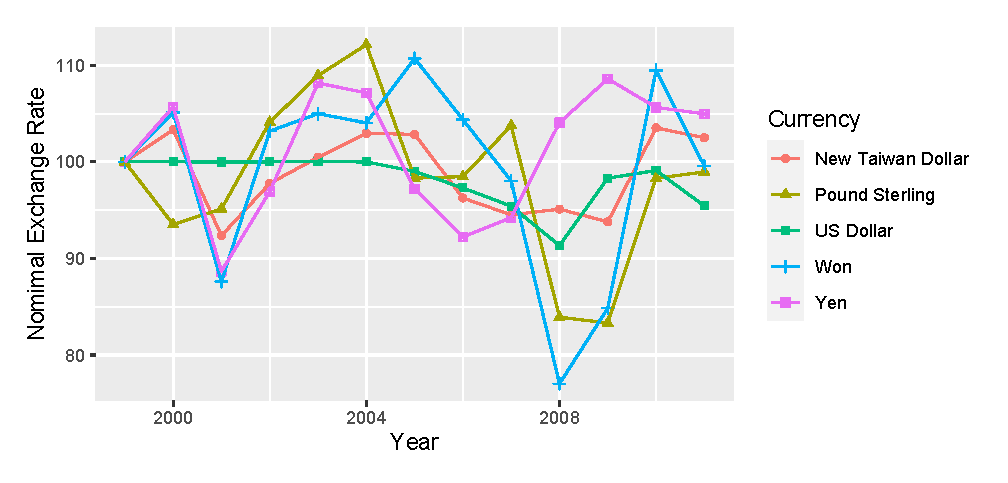
\includegraphics[width=1\textwidth]{figure/figure1.eps}
	\caption{Nominal exchange rates of China's major trading partners (1999-2011)}
	\label{fig3.1}
\end{figure}

\begin{figure}[htbp]
	\centering
	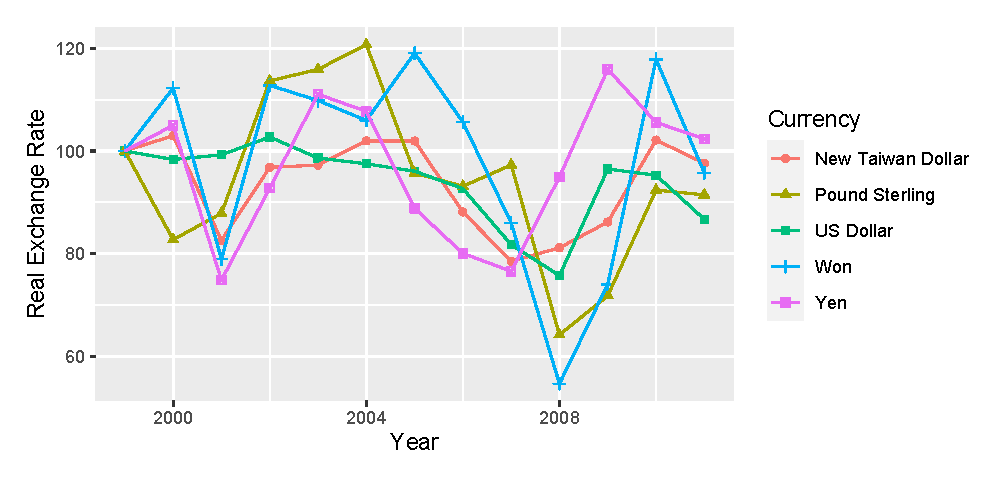
\includegraphics[width=1\textwidth]{figure/figure2.eps}
	\caption{Nominal exchange rates of China's major trading partners (1999-2011)}
	\label{fig3.2}
\end{figure}
